\section{Introduction}

With the in-depth research on networked multi-agent technology, multi-robot systems (MRSs) have rapidly developed towards autonomy, offering various applications in various areas over the last few decades~\cite {6303906,1335496}. In multi-robot control, formation control plays a crucial key technology, in which robots are required to form and maintain a desired configuration~\cite{1545539,Oh2015}. In fixed-configuration formation control, achieving the desired configuration involves setting a specific target distance for each swarm agent. However, with the increasing diversity and complexity of formation tasks, it is crucial to adjust the formation method based on specific task requirements in real-time. Consequently, time-varying formation (TVF) control has become essential for practical robot applications~\cite{Dong2015,Dong2016}.

Research in~\cite{736776,Reynolds1987,Antonelli2009} proposed that the motion of a biological swarm can be described by the combination of three behavioral rules, including (i) cohesion, which brings each agent closer to its neighbors, (ii) repulsion, which drives each agent away from its neighbors to avoid collisions, and (iii) alignment, which steers each agent towards the average heading of its neighbors. These rules apply to each agent simultaneously. In goal-oriented swarm flight, alignment behavior is replaced by migration behavior, guiding each UAV in a desired migration direction with a preferred speed~\cite{6095129}. In the obstacle environments, the navigation of a UAV swarm can be enhanced by introducing a fourth behavior, collision avoidance, which navigates UAVs around obstacles~\cite{9565893,9990164,1605401,10417519}. Mathematically, these rules can be modeled using virtual forces with potential fields, which encode the desired behaviors of the swarm.

\begin{figure}
\centering
\begin{subfigure}[b]{0.4\textwidth}
    
    \centering
    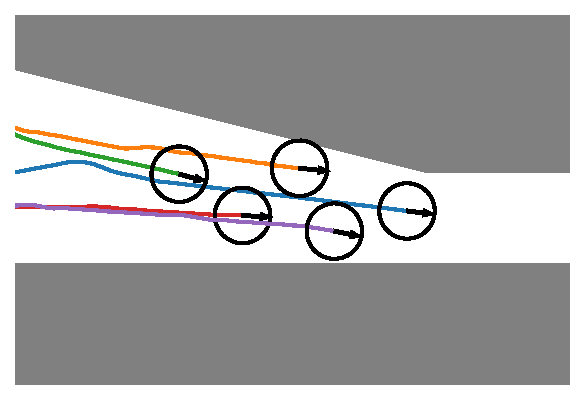
\includegraphics[width=\linewidth]{paper2/images/sample_bc.pdf}
    \caption{Pure formation control}
    \label{fig:1sample_bc}
\end{subfigure}
\begin{subfigure}[b]{0.4\textwidth}
    \centering
    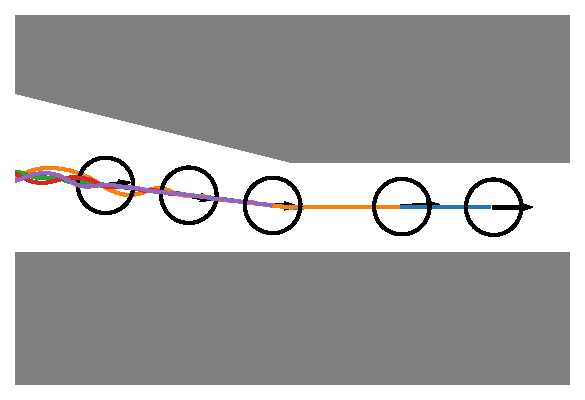
\includegraphics[width=\linewidth]{paper2/images/sample_edc.pdf}
    \caption{Proposed approach}
    \label{fig:1sample_edc}
\end{subfigure}
\caption{We develop an event-based formation reconfiguration control method to guide a TVF through confined spaces, including narrow gaps. \textit{Left:} Motion path of the TVF using purely behavior-based formation control~\cite{736776, Vsrhelyi2018}, which are collisions with surrounding obstacles. \textit{Right:} Motion path of the TVF using our proposed approach, which safely navigates through the narrow gap.}
\label{fig:1sample}
\end{figure}

Based upon the behavioral control method, authors in~\cite{8716301} successfully applied a strategy for multi-robot systems maintaining the global network integrity by putting constraints on the movement at each step and removing redundant connectivity.  With the advantage of low computational complexity~\cite{1605401,Reynolds1987}, the potential field offers practical implementation in real robot systems across various environmental conditions, from free space~\cite{Reynolds1987} to environments with convex or concave obstacles~\cite{10417519,9565893}. Inspired by biological swarms, the coordinated and synchronized motion of the robot swarm can effectively address unforeseen situations and complex environments with dense obstacles, such as forest-like settings~\cite{9981858, 9561902, 9990164}. However, the cave-like scenarios have not received much attention, i.e. the environment is not enough to maintain the desired configuration. Passing through a narrow environment, e.g. caves, corridors, narrow passages, and so on~\cite{Dang2020,9220149} is still considered a crucial challenge for swarm navigation in general and formation control in particular, because maintaining a rigid formation~\cite{736776} when moving through narrow spaces poses many risks of collision. As a result, local minima often occur when a robot formation moving through a narrow environment cannot maintain formation while avoiding collisions with the surrounding environment~\cite{Saska2020}.

Within the domain of formation control, numerous approaches have been devised to facilitate the safe navigation of multi-robot formations through obstacle environments~\cite{Saska2020,Gmez2013,Ebel2017,Roy2018,AlonsoMora2017,Fu2020,8843165,Vsrhelyi2018}. This research domain is predominantly categorized into two primary types: \textit{formation maintenance}, where the original shape remains unchanged or contract/expand the configuration over time~\cite{Saska2020,Gmez2013,Ebel2017,Roy2018}; and \textit{formation transformation}, where the formation can transform to another configuration upon encountering obstacles~\cite{AlonsoMora2017,Fu2020,8843165}.

In the context of \textit{formation maintenance}, the formation consistently maintains its desired shape or realigns via shrink/expand configuration during movement. In~\cite{Saska2020}, a model predictive control is employed to provide optimal control signals for each robot information based on the sharing of map updates. As a result, the amount of communication between them became significant, facing communication delays as the number of members in the formation increased. A region-based hierarchical control employed in~\cite{Roy2018} addresses obstacle-avoidance challenges in the virtual structure when moving through confined spaces. Here, robots move cohesively within a circular region, which can contract to avoid obstacles. Nevertheless, approaches in this case become more challenging in maintaining a predetermined formation in confined environments, as described in Fig.~\ref{fig:1sample}. This challenge arises significantly when the contraction of the formation heightens the risk of collisions among individuals and the surrounding space.

The second case, \textit{formation transformation} involves the flexible transformation of the configuration into a distinct configuration to effectively navigate threats. The work in~\cite{Fu2020} introduces a formation maintenance and restructuring strategy combining behavioral control with obstacle velocity techniques to adeptly navigate dynamic environments. This restructuring strategy decided based on an auction-based market approach, presents an optimal solution for effective formation movement. However, communication costs are considerable, and communication between robots must be carried out continuously to make the optimal target decisions for each individual. An algorithm based on particle swarm optimization for the reconfigurable formation of multiple UAVs for visual inspection is introduced in~\cite{8843165}. The flight path is constructed, accounting for visual inspection constraints, and a reconfigurable topology is introduced to enable obstacle collision avoidance during operation. However, this centralized approach needs resources to obtain the optimal configuration at each time, which leads to challenges for robustness and scalability.

To the best of the authors' knowledge, our study constructs a strategy that can dynamically change formations based on calculations sensed from the environment. The changing decision signal is event-triggering and at a lower computational cost. Of these few existing studies, some studies use centralized control to construct control strategies~\cite{Gmez2013,Roy2018,AlonsoMora2017,8843165} or the information communicated between individuals is very large~\cite{Saska2020,Fu2020}. Our solution is fully distributed control and the amount of communication information between individuals is lightweight, only including position and velocity information. In addition, when transforming to another configuration, the order of each member is calculated reasonably and is not pre-arranged, ensuring reconfiguration takes place safely and immediately.

Motivated by the limitations of the mentioned issues, this paper proposes an event-based formation reconfiguration control strategy for a TVF to pass through confined space environments, as given in Fig.~\ref{fig:1sample}. The approach utilizes potential field techniques to design the behaviors of formation. The event-based mode-switching strategy is then presented based on the individual sensing capacity in formation. The main contributions of our work are threefold:
\begin{enumerate}
    \item Propose an event-based formation reconfiguration control strategy designed to enable the formation to scale, and transform to a straight line configuration, allowing it to effectively adapt to safely traverse confined environments;
        \item Design behaviors for the TVF based on potential field function and demonstrate the stability of the control law through Lyapunov theorem;
    \item Validate the proposed method through numerous simulations and comparisons. Software-in-the-loop (SIL) experiments are also conducted to evaluate the effectiveness.
\end{enumerate}

The remaining sections of this paper are constructed as follows. Section \ref{sec2} covers preliminaries and problem formulation. Section \ref{sec3} presents the proposed distributed control strategy to reconfigure the formation to prevent collision with the environment. The proposed method is illustrated through simulation results and evaluation metrics in Section \ref{sec4}. Section \ref{sec5} ends the paper with conclusions.

